\documentclass[a4paper, 12pt]{article}
\usepackage[T1]{fontenc}
\usepackage{lmodern}
\usepackage{color}
\usepackage{amsfonts}
\usepackage{epstopdf}
\usepackage{matlab}
\usepackage{booktabs}
%\documentclass{book}
\usepackage{blindtext}
\usepackage{hyperref}
\usepackage[brazil]{babel}
\usepackage{amssymb}
\usepackage[utf8]{inputenc}
\usepackage{amsmath}
\usepackage{indentfirst}
\usepackage{graphicx}
\usepackage{listings}
\usepackage{tcolorbox}
\usepackage{upgreek}
\usepackage{multicol,lipsum}
\usepackage[a4paper,
top=3cm, left=3cm, bottom=3cm, right=3cm]{geometry}
\usepackage{setspace}
\usepackage{multirow}
\usepackage{float}
\usepackage[dvipsnames]{xcolor}
\usepackage[table]{xcolor}
%\usepackage{pdflscape}
\usepackage[DIV=15]{typearea}
\usepackage[nottoc]{tocbibind}
\usepackage[sort,numbers]{natbib}
%\usepackage{cite}
\usepackage{matlab}

\usepackage[utf8]{inputenc}
\usepackage[T1]{fontenc}
\usepackage{lmodern}
\usepackage{graphicx}
\usepackage{color}
\usepackage{hyperref}
\usepackage{amsmath}
\usepackage{amsfonts}
\usepackage{epstopdf}
\usepackage[table]{xcolor}
\usepackage{matlab}





\documentclass[letterpaper]{article}
% bib pack %%%%%%%%%%%%%%%%%%%%%%%%%%%%%%%%%%%%%%%%%%%%%%%%%%%%%%%%%%%%%%%%%%%%%
\usepackage[utf8]{inputenc}
\usepackage{geometry}
    \geometry{left=3cm,right=2cm,top=2cm,bottom=2cm}
%
\usepackage[spanish]{babel}
%
\usepackage[fixlanguage]{babelbib}
    \bibliographystyle{babunsrt}
%
\usepackage{url}

\begin{document}
%\maketitle

\begin{titlepage}
	\begin{center}
		

\vspace{10pt}
%\begin{figure}[H][!ht]
%\centering
%
\includegraphics{puc-rio-logo.png}

%\end{figure}
\begin{figure}[!ht]
\centering

\includegraphics{images/puc-rio-logo.png}
\end{figure}
\huge{Otimização: Algoritmos e Aplicações na Engenharia}
        \vspace{70pt}
        
		\textbf{MEC2403}
		\textbf{\large{\\ }}
		
		\vspace{30pt}
		\textbf{\small{\\Lista 02}}
		\vspace{75pt}
		
	\end{center}
	
	\begin{flushleft}
		\begin{tabbing}
		Alunos\qquad\qquad\=\>Paloma Sette - 1621595\\
			
			Professor(a)\>Ivan Menezes\\
	\end{tabbing}
		  
	\end{flushleft}
	\begin{center}
		%\vspace{\fill}
		\vspace{215pt}
		Rio de Janeiro, 17 de Setembro de 2024
	\end{center}
\newpage
\tableofcontents
\thispagestyle{empty}

\newpage
\pagenumbering{arabic}

\newpage

%\newcommand{\listequationsname}{Lista de Equações}
%\newlistof{myequations}{equ}{\listequationsname}
%\newcommand{\myequations}[1]{%
%\addcontentsline{equ}{myequations}{\protect\numberline{\theequation}#1}\par}

%\listofmyequations
\newpage


\newpage

\listoffigures
\thispagestyle{empty}

\newpage
%%%%%%%%%%%%%%%%%%%%%%%%%%%%%%%%%%%%%%%%%%%%%%%%%%%%%%%%%
%%%%%%%%%%%%%%%%%%%%%%%%%%%%%%%%%%%%%%%%%%%%%%%%%%%

\newpage

\thispagestyle{empty}

\newpage


\section{Questão 01}
Devemos implementar, utilizando o MATLAB, os seguintes métodos para cálculo do ponto de mínimo de funções de uma única variável: \\


\bullet \>\ Passo \>\ constante \>\ (com \>\ $\Delta \alpha = 0.01$);\\
\bullet \>\ Bisseção;\\
\bullet \>\ Seção \>\ Áurea;\\

%\subsection{Passo Constante}

\subsection{Bisseção}

\sloppy
\epstopdfsetup{outdir=./}
\graphicspath{ {./L01_Latex_images/} }


\begin{matlabcode}

function [aM] = Bissecao( x0, d, aL, aU, TOL, item)

eps = 1e-5;

erro = abs ( aU - aL );

while ( erro >= TOL )
    aM = ( aL + aU ) / 2;   
    f1 = FuncaoObjetivo ( x0, d, (aM-eps), item);
    f2 = FuncaoObjetivo ( x0, d, (aM+eps), item);
	if f1 > f2
        aL = aM;
    else
        aU = aM;
    end
    erro = abs ( aU - aL );
end
aM = ( aL + aU ) / 2;

end

\end{matlabcode}

\subsection{Seção Áurea}

\sloppy
\epstopdfsetup{outdir=./}
\graphicspath{ {./L01_Latex_images/} }


\begin{matlabcode}

function [a] = SecaoAurea( x0, d, aL, aU, TOL )

% Razão Áurea
RA = ( sqrt(5) - 1) / 2;

% "Tamanho" do intervalo
beta = abs ( aU - aL );

% Pontos "intermediários" do intervalo
aE = aL + ( 1 - RA ) * beta;   
aD = aL +  RA * beta;   
fE = FuncaoObjetivo ( x0, d, aE );
fD = FuncaoObjetivo ( x0, d, aD );

while ( beta >= TOL )
	if fE > fD
        aL = aE;
        aE = aD;
        fE = fD;
        beta = abs ( aU - aL );
        aD = aL +  RA * beta;
        fD = FuncaoObjetivo ( x0, d, aD );
    else
        aU = aD;
        aD = aE;
        fD = fE; 
        beta = abs ( aU - aL );
        aE = aL +  ( 1 - RA ) * beta;
        fE = FuncaoObjetivo ( x0, d, aE );
    end
end
a = ( aL + aU ) / 2;

end

\end{matlabcode}


\subsection{Passo Constante}
\begin{matlabcode}

function [aL,aU] = PassoConstante( x0, d, DeltaAlpha )

% Calcula o valor da Função no Ponto Inicial
alpha = 0;
f0 = FuncaoObjetivo ( x0, d, alpha );

% Verifica o sentido positivo da busca
eps = 1e-6;

f1 = FuncaoObjetivo ( x0, d, eps );

dir = d;
flagdir = 1;
if f1 > f0
   dir = -d;
   flagdir = -1;
end

while 1
   alpha = alpha + DeltaAlpha;
   f = FuncaoObjetivo ( x0, dir, alpha );
   f1 = FuncaoObjetivo ( x0, dir, (alpha-eps) );
   if  f1 < f
      aL = alpha - DeltaAlpha;
	  aU = alpha;
	  break;
   end
end

if flagdir == -1
   temp = aL;
   aL = -aU;
   aU = -temp;
end

end

\end{matlabcode}


\newpage
\section{Questão 02}

Com os métodos implementados anteriormente, devemos testar encontrando o ponto de mínimo das seguintes funções especificadas nos tópicos seguintes.

\subsection{Primeira Função}

\begin{equation}
    f(x_1, x_2) = x_1^2 - 3x_1x_2 + 4x_2^2 + x_1 - x_2
\end{equation}

\begin{center}
    Ponto Inicial: $x^0 = \{1,2\}^t$ \>\ \>\ Direção: $d = \{-1,-2\}^t$
\end{center} \\

Ao aplicarmos os métodos implementados, foram encontrados os seguintes valores pelo MATLAB:

\begin{figure}[H]
\centering
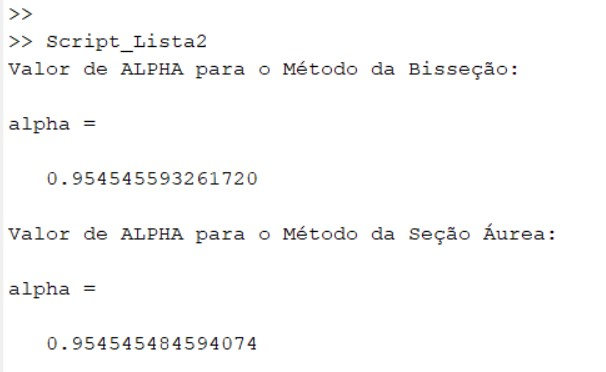
\includegraphics[scale = 0.7]{images/resultados_A.jpg}
\caption{Resultados - Primeira Função}
\end{figure}

A partir de então, foi implementado o seguinte código para obtenção do gráfico e das curvas de nível: 

\begin{matlabcode}
    % Parâmetros
x0 = [1; 2];  % Ponto inicial
d = [-1; -2];  % Direção
alpha_bissecao = 0.954545593261720;  % Valor de alpha 
pelo método da bisseção

alpha_secao_aurea = 0.954545484594074;  % Valor de alpha 
pelo método da Seção Áurea

% Ponto de mínimo (usando o valor de alpha da bisseção, por exemplo)
x_min = x0 + alpha_bissecao * d;

% Criando uma malha de valores para plotar as curvas de nível
[X1, X2] = meshgrid(-1:0.1:3, -1:0.1:3);  
% Ajuste o intervalo conforme necessário

% Função objetivo
F = X1.^2 - 3 .* X1 .* X2 + 4 .* X2.^2 + X1 - X2;

% Plotando as curvas de nível
contour(X1, X2, F, 50);  % 50 curvas de nível
hold on;

% Plotando o ponto inicial e o ponto de mínimo
plot(x0(1), x0(2), 'ro', 'MarkerSize', 
8, 'MarkerFaceColor', 'r');  % Ponto inicial
plot(x_min(1), x_min(2), 'bo', 
'MarkerSize', 8, 'MarkerFaceColor', 'b');  % Ponto de mínimo

% Plotando o segmento de reta entre o ponto inicial e o ponto de mínimo
plot([x0(1), x_min(1)], [x0(2), x_min(2)], 'k-', 'LineWidth', 2);  
% Segmento de reta

% Labels e título
xlabel('x_1');
ylabel('x_2');
title('Curvas de Nível e Segmento de Reta');
legend('Curvas de Nível', 
'Ponto Inicial', 'Ponto de Mínimo', 
'Segmento de Reta');

hold off;

\end{matlabcode}


O gráfico abaixo apresenta as \textbf{curvas de nível} da função \( f(x_1, x_2) = x_1^2 - 3x_1x_2 + 4x_2^2 + x_1 - x_2 \), representando as regiões onde a função mantém um valor constante. Essas curvas ilustram a topografia do problema de otimização, facilitando a visualização do comportamento da função em diferentes áreas do espaço de busca.\\

Além das curvas de nível, foi plotado o \textbf{segmento de reta} que conecta o \textbf{ponto inicial} \( x_0 = [1; 2] \) ao \textbf{ponto de mínimo} \( x_{\text{min}} \), encontrado utilizando o método de \textbf{Bisseção}. O ponto de mínimo foi determinado ao longo da direção \( d = [-1; -2] \), com o valor ótimo de \( \alpha \) resultante de \( \alpha_{\text{bisseção}} \approx 0.9545 \). O ponto inicial está representado em \textbf{vermelho}, enquanto o ponto de mínimo está indicado em \textbf{azul}. O segmento de reta preto mostra o caminho percorrido pela otimização unidimensional na direção de busca definida.\\

Observa-se que o método foi eficiente na convergência para o mínimo local da função, o qual está em uma região de concentração das curvas de nível, indicando o ponto de menor valor da função dentro do intervalo definido.


\begin{figure}[H]
\centering
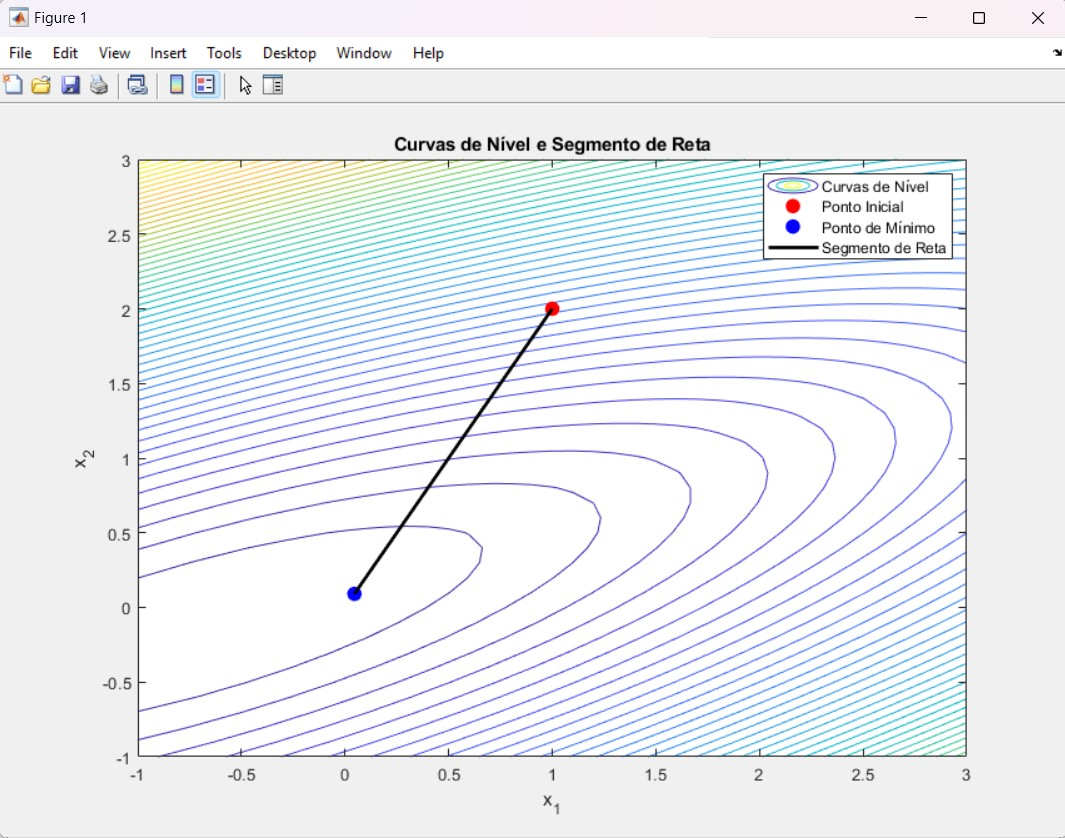
\includegraphics[scale = 0.6]{images/figura_A.jpg}
\caption{Curvas de nível primeira função da questão 2}
\end{figure}




\newpage
\subsection{Função de McCormick}

\begin{equation}
    f(x_1, x_2) = sin(x_1+x_2) + (x_1-x_2)^2 - 1.5x_1 + 2.5x_2
\end{equation}


\begin{center}
    Ponto Inicial: $x^0 = \{-2,3\}^t$ \>\ \>\ Direção: $d = \{1.453,-4.547\}^t$
\end{center}

Os resultados abaixo foram gerados pelo MATLAB:

\begin{figure}[H]
\centering
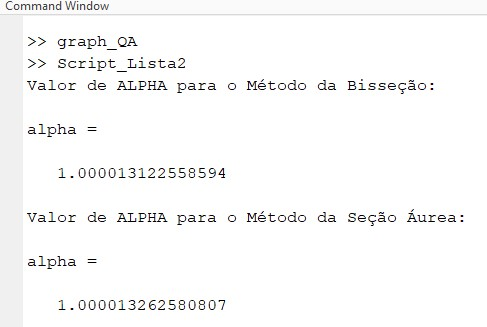
\includegraphics[scale = 0.7]{images/resultados_B.jpg}
\caption{Resultados para a função de McCormick}
\end{figure}

Utilizando o mesmo código implementado no item (a), alterando apenas os parâmetros, obtivemos o seguinte:

\begin{figure}[H]
\centering
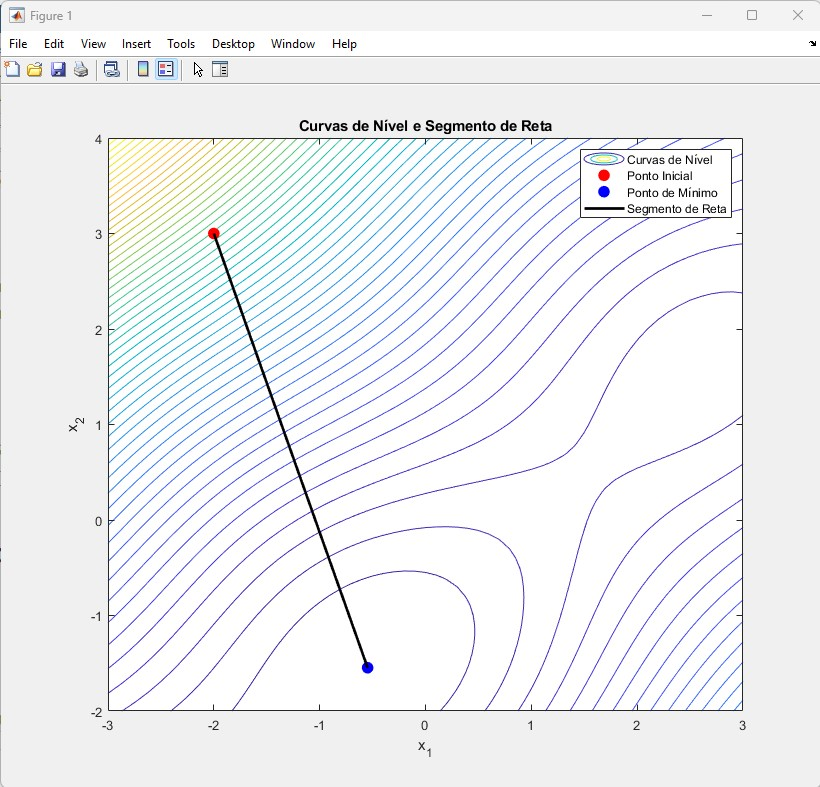
\includegraphics[scale = 0.7]{images/figura_B.jpg}
\caption{Curvas de nível função da questão 2 - McCormick}
\end{figure}


O gráfico acima ilustra as \textbf{curvas de nível} da função de McCormick, definida como:

\[
f(x_1, x_2) = \sin(x_1 + x_2) + (x_1 - x_2)^2 - 1.5 \cdot x_1 + 2.5 \cdot x_2
\]

As curvas de nível representam regiões de valor constante da função no plano \(x_1\)-\(x_2\), fornecendo uma visão do comportamento da função ao longo da área de busca. \\

O \textbf{ponto inicial} foi definido como \( x_0 = [-2; 3] \), e a otimização foi realizada ao longo da direção \( d = [1.453; -4.547] \). O \textbf{ponto de mínimo} foi determinado usando o valor de \( \alpha \) obtido pelo método de \textbf{Bisseção}, resultando em \( \alpha_{\text{bisseção}} \approx 1.0000 \). O ponto de mínimo está localizado em \( x_{\text{min}} = [-0.5367; -1.4817] \), representado no gráfico pelo marcador em \textbf{azul}.\\

O \textbf{segmento de reta} preto conecta o ponto inicial ao ponto de mínimo, ilustrando o caminho percorrido ao longo da direção de busca durante o processo de otimização. O comportamento da função, bem como a convergência para o mínimo local, são adequadamente representados pelas curvas de nível concêntricas ao redor do ponto de mínimo.\\



\newpage
\subsection{Função de Himmelblau}

\begin{equation}
    f(x_1, x_2) = (x_1^2 + x_2 - 11)^2 + (x_1 + x_2^2 - 7)^2
\end{equation}


\begin{center}
    Ponto Inicial: $x^0 = \{0,5\}^t$ \>\ \>\ Direção: $d = \{3, 1.5\}^t$
\end{center}

Pelo MATLAB, obtivemos o seguinte resultado para os valores de 
 $\alpha$:
 
\begin{figure}[H]
\centering
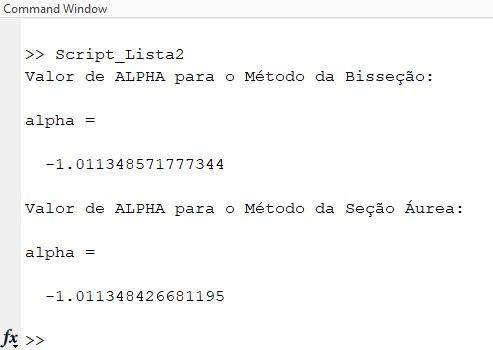
\includegraphics[scale = 0.8]{images/resultados_C.jpg}
\caption{Resultados para a função de Himmelblau}
\end{figure}

A partir de então, utilizando o código demonstrado em (a) e alterando os parâmetros necessários, geramos as curvas:


\begin{figure}[H]
\centering
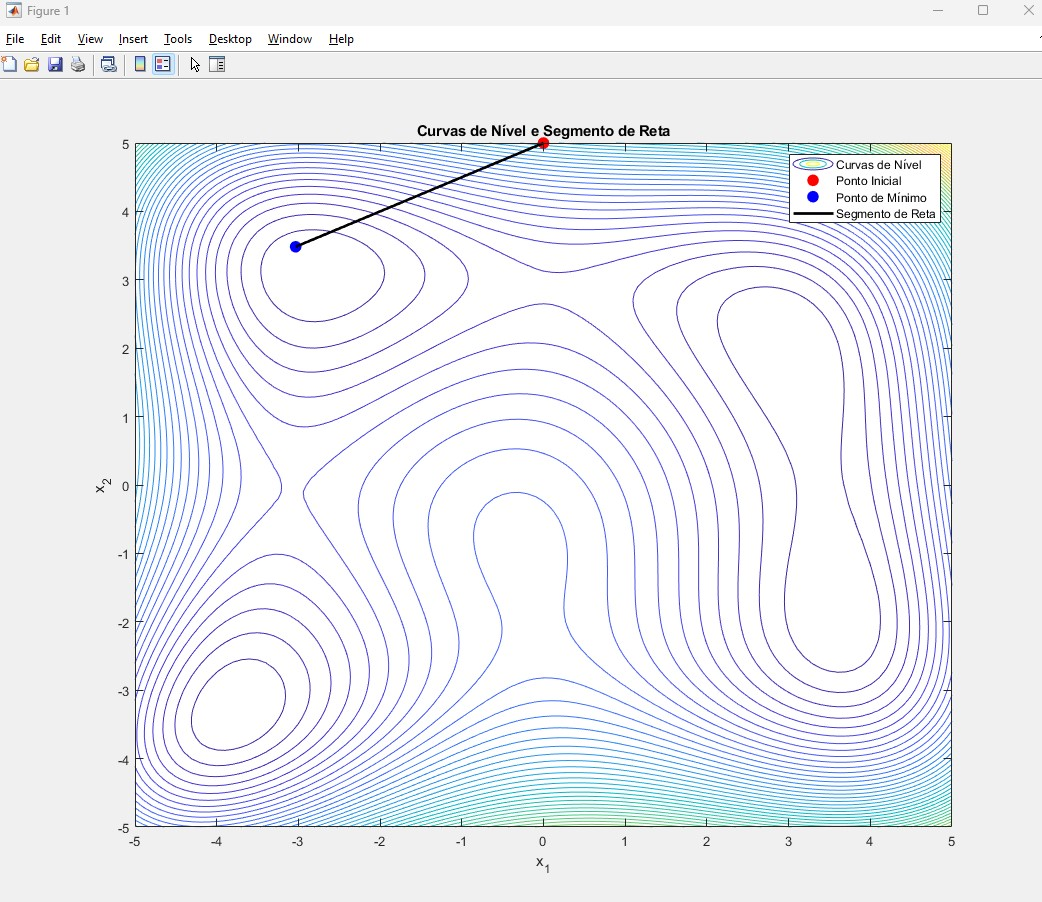
\includegraphics[scale = 0.6]{images/figura_C.jpg}
\caption{Curvas de nível da função de Himmelblau}
\end{figure}


Portanto, gráfico acima apresenta as \textbf{curvas de nível} da função de Himmelblau, definida como:

\[
f(x_1, x_2) = (x_1^2 + x_2 - 11)^2 + (x_1 + x_2^2 - 7)^2
\]

As curvas de nível ilustram as regiões de valor constante da função no plano \(x_1\)-\(x_2\), permitindo uma visualização da topografia da função objetivo.\\

O \textbf{ponto inicial} foi definido como \( x_0 = [0; 5] \), e a otimização foi realizada ao longo da direção \( d = [3; 1.5] \). O \textbf{ponto de mínimo} foi encontrado utilizando o valor de \( \alpha \) obtido pelo método de \textbf{Bisseção}, resultando em \( \alpha_{\text{bisseção}} \approx -1.0113 \). O ponto de mínimo foi localizado em \( x_{\text{min}} = [-3.034; 3.483] \), representado no gráfico pelo marcador em \textbf{azul}.\\

O \textbf{segmento de reta} preto conecta o ponto inicial ao ponto de mínimo, mostrando o caminho percorrido ao longo da direção de busca durante o processo de otimização. As curvas de nível revelam o comportamento da função e a concentração ao redor do ponto de mínimo, ilustrando a convergência do método para a solução ótima.




\newpage
% REFERENCIAS %%%%%%%%%%%%%%%%%%%%%%%%%%%%%%%%%%%%%%%%%%%%%%%%%%%%%%%%%%%%%%
    \nocite{*}
    \bibliography{src/bibliography}
    

\section{Referências Bibliográficas}

\end{document}